\section{Fusion}
Kärnreaktorer har ni säkert hört talas om. Oftast funkar dessa genom att klyva atomkärnor, det vill säga utföra \emph{fission}. Stjärnor gör något liknande, men de sätter ihop atomkärnor i stället för att klyva isär dem. Detta heter \emph{fusion}. Det krävs väldigt högt tryck och temperatur för att möjliggöra fusion, men i vissa fall ger processen mer energi ut än som sattes in, vilket är det som bland annat möjliggör stjärnor.

Både fission och fusion fungerar eftersom olika atomer har olika \emph{bindningsenergi}. Det finns nämligen en viss energi som krävs för att se till att nukleonerna i atomkärnan inte flyger iväg. Bindningsenergin är också förvånansvärt stor. Vi har svårt att mäta den direkt, men man kan använda Einsteins materia-energiekvivalens:
\begin{equation}
    E = mc^2
    \label{eq:emc2}
\end{equation}
i stället.

Ekvivalensen säger att den totala energin lagrat i ett visst föremål är lika med dess massa gånger ljusets hastighet i kvadrat. Med hjälp av detta kan vi observera skillnaden i energi mellan samma molekyl i olika tillstånd. Till exempel kommer energin för 2 lösa protoner (\ce{2p+}) och 2 lösa neutroner (\ce{2n}) vara större än dessa sammansatta för att bilda en \ce{^2_4He^2+} kärna som ni kan se i \cref{tab:helium-energy}. Beräkningen här utgår från de uppmätta massorna för protoner, neutroner och heliumkärnan. En elektrons massa är försumbart liten i detta sammanhang, och deltar därför inte i beräkningarna.

Denna relation kan även tillämpas för skillnaden mellan två fria atomkärnor och en större atomkärna bildad genom att \emph{fusionera} --- sätta samman till ett --- de två kärnorna. För lika par av grundämnen gäller det att deras fusionsprodukt alltid har lite lägre total bindningsenergi än de skilda upp till järnatomen. Efter järn, på grund av kvantmekaniska effekter, ökar bindningsenergin för varje tillsatt nukleon. Varför det är så är utanför nivån av denna föreläsning. Bindningsenergierna för varje tillsatt nukleon finns illustrerat i \cref{fig:binding-energy}. Lägg märke till att även litium förlorar energi och därmed hoppas över i stjärnfusion så att man går direkt till kol från helium.

\begin{figure}
    \centering
    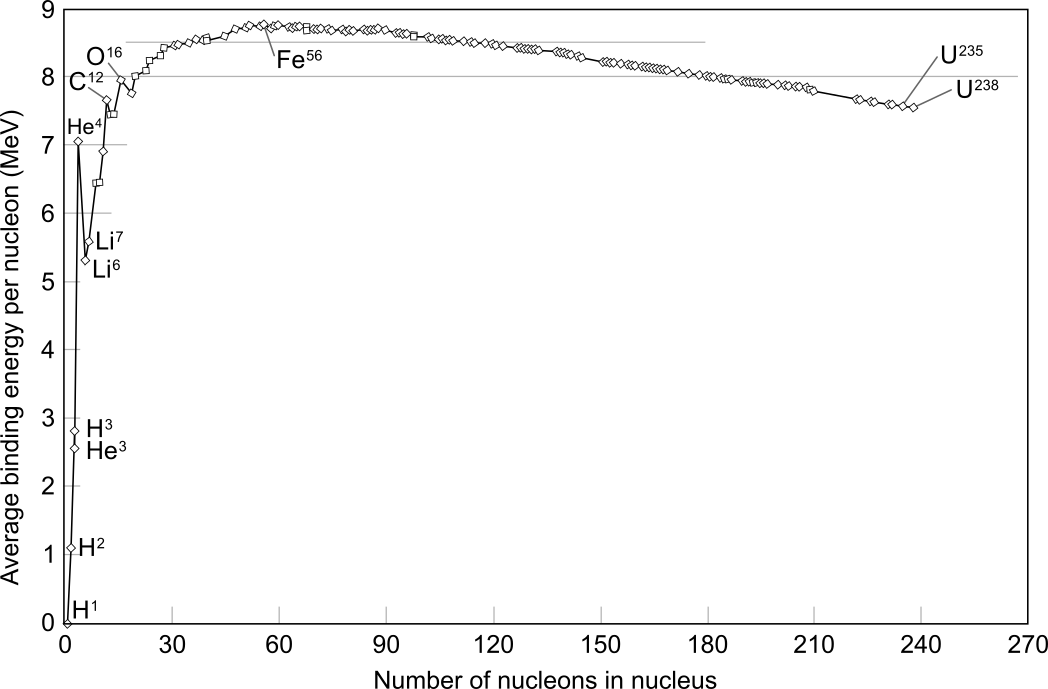
\includegraphics[width=0.75\textwidth]{img/Binding_energy_curve_-_common_isotopes.png}
    \caption{Bindningsenergi per nukleon för olika atomkärnor.}
    \label{fig:binding-energy}
\end{figure}

Detta innebär i slutändan att fusionsreaktioner av lika atompar ger ett energiöverskott för grundämnen upp till järn. Överskottet blir till värme när fusionen är klar. Den extra energin är ganska liten jämfört med energin som krävs för att trycka ihop atomkärnorna men är inte försumbar i stora skalor med många atomer samtidigt. För fusion av olika par är frågan mer komplicerad, men generellt sett är det energivinst även där upp till järn.

\subsection{Fusion i stjärnor}
Tack vare stjärnors stora tryck, och temperatur, möjliggör en stjärna med stor nog massa fusion av grundämnen. Ju större massa, desto varmare blir det och desto mer kan man fusionera. Detta beror på trycket från gravitationen. Gränsen för att kunna fusionerna väte till helium ligger på \qty{\sim 0.08}{\Mo}\footnote{Källa: \textcolor{blue}{\url{https://sites.uni.edu/morgans/astro/course/Notes/section2/fusion.html}}} (solmassor). Sedan finns det en skala för hur mycket energi, och därav massa hos stjärnan, krävs för att fusionera varje element. Till slut når man kisel till järn fusion, och därefter är energipositiv fusion omöjlig. Detta innebär också att järn inte längre kan fusioneras av stjärnan.

Fusion i stjärnor är inte lika perfekt som min tidigare förklaring antydde. Det är sällan lika atompar som bara sådär slås samman. Exempelvis finns proton-proton fusion som skapar helium från väten som ni kan se i \cref{fig:proton-proton}. Det är denna process som just nu pågår i solen.

\begin{figure}
    \centering
    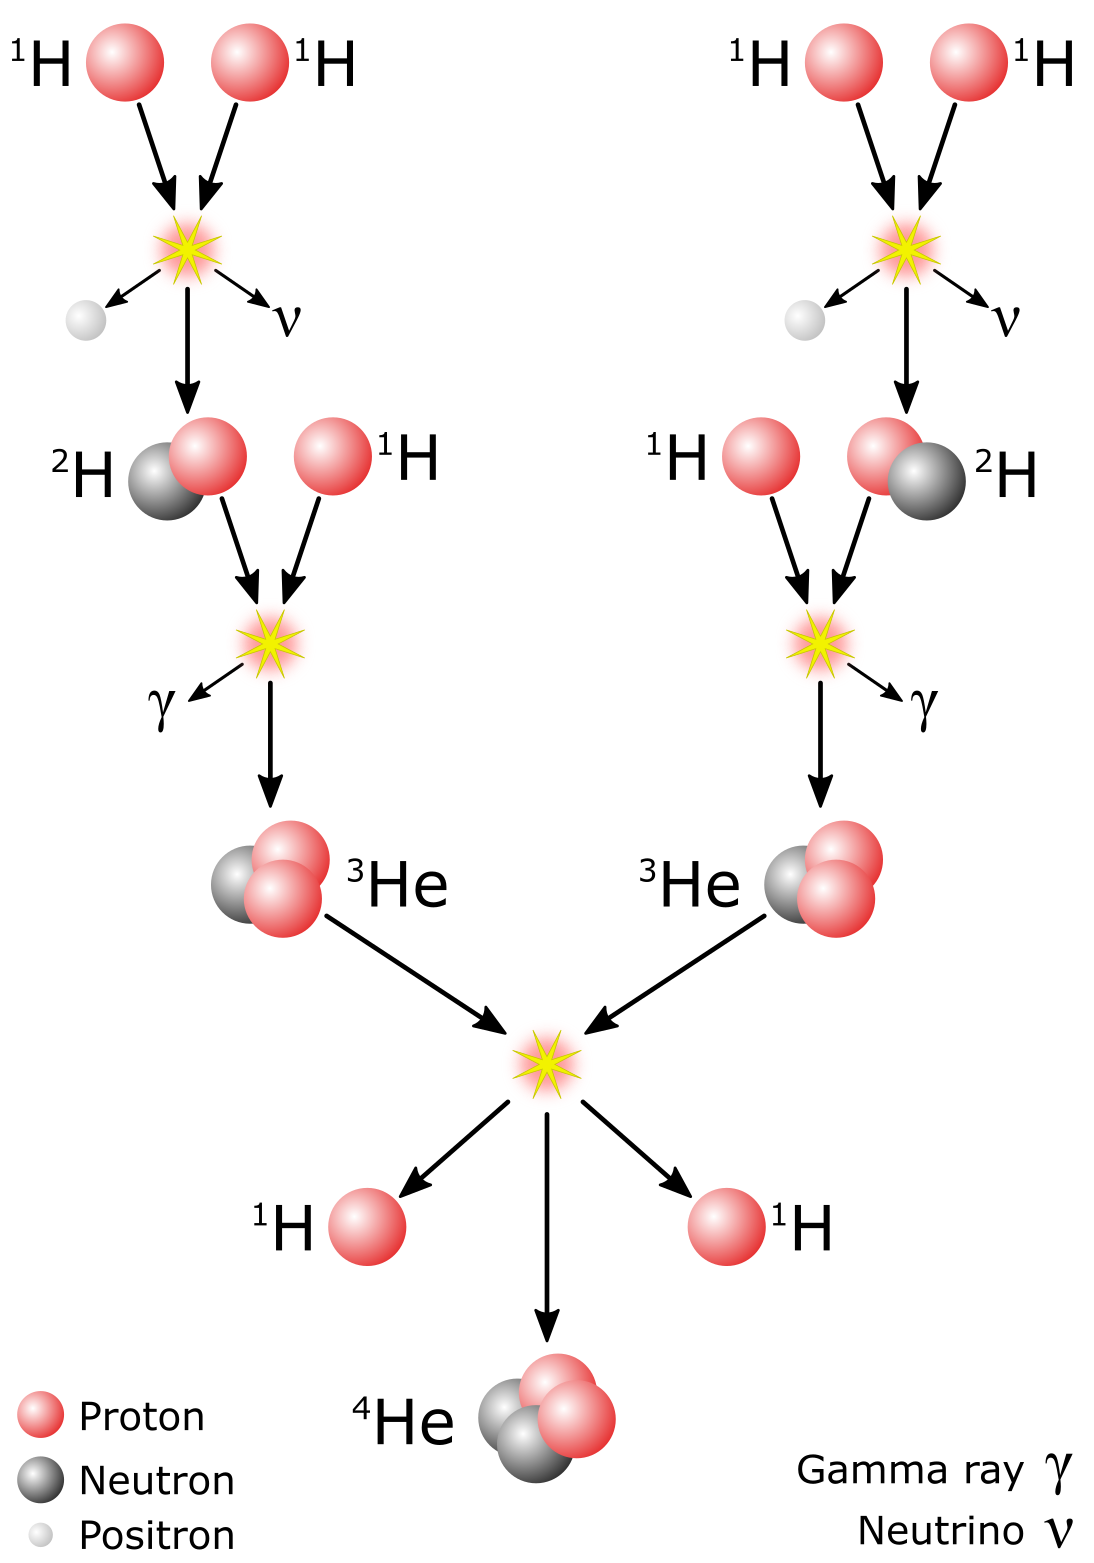
\includegraphics[width=0.35\textwidth]{img/Fusion_in_the_Sun.png}
    \caption{Proton-proton fusion.}
    \label{fig:proton-proton}
\end{figure}

\begin{table}[b]
    \def\arraystretch{1.5}
    \centering
    \caption{Energin för heliums beståndsdelar och dess kärna.}
    \label{tab:helium-energy}
    \begin{tabular}{c|c|c}
        \textbf{Sak} & \textbf{Massa (kg)} & \textbf{Energi (J)} \\\toprule
        \ce{2p+ + 2n} & \qty{6.696e-27}{kg} & \qty{6.018e-10}{J}\\
        \ce{^2_4He^2+} & \qty{6.646e-27}{kg} & \qty{5.974e-10}{J} \\\bottomrule
        \textbf{Differens} & \qty{5e-30}{kg} & \qty{4.4e-12}{J}

    \end{tabular}
\end{table}

\section{Stjärnornas anatomi}
En stjärna är i grund och botten en boll av gas. Först och främst består dem av väte (\ce{H}) och helium (\ce{He}). De innehåller dock ämnen hela vägen upp till järn (\ce{Fe}) i periodiska systemet (se \vref{fig:periodic-table} för ett periodiskt system). De allra första stjärnorna vara i princip bara väte och helium, men nästa generation av stjärnor bildades av gas från den exploderade förra generationen. Den gasen innehåller många tyngre ämnen som bildats och därmed tillförts den nya stjärnan.

Deras inre struktur kan liknas till en lök. Ju större, och äldre, en stjärna är desto fler lager har den. Man kan betrakta stjärnan som en fusionerande kärna och ett icke-fusionerade yttre lager samt en atmosfär. ''Kärnan'' är ett missvisande begrepp här, eftersom det som faktiskt kallas \emph{kärna} är endast det innersta lagret. Dock finns det i äldre stjärnor fusionerande lager runt kärnan. Atmosfären är distinkt från det icke-fusionerande lagret eftersom den är genomskinlig för ljus, till skillnad från de inre lagren. Ett diagram för en äldre stjärna av stor massa finns i \cref{fig:star-anatomy}.
\begin{figure}[h!]
    \centering
    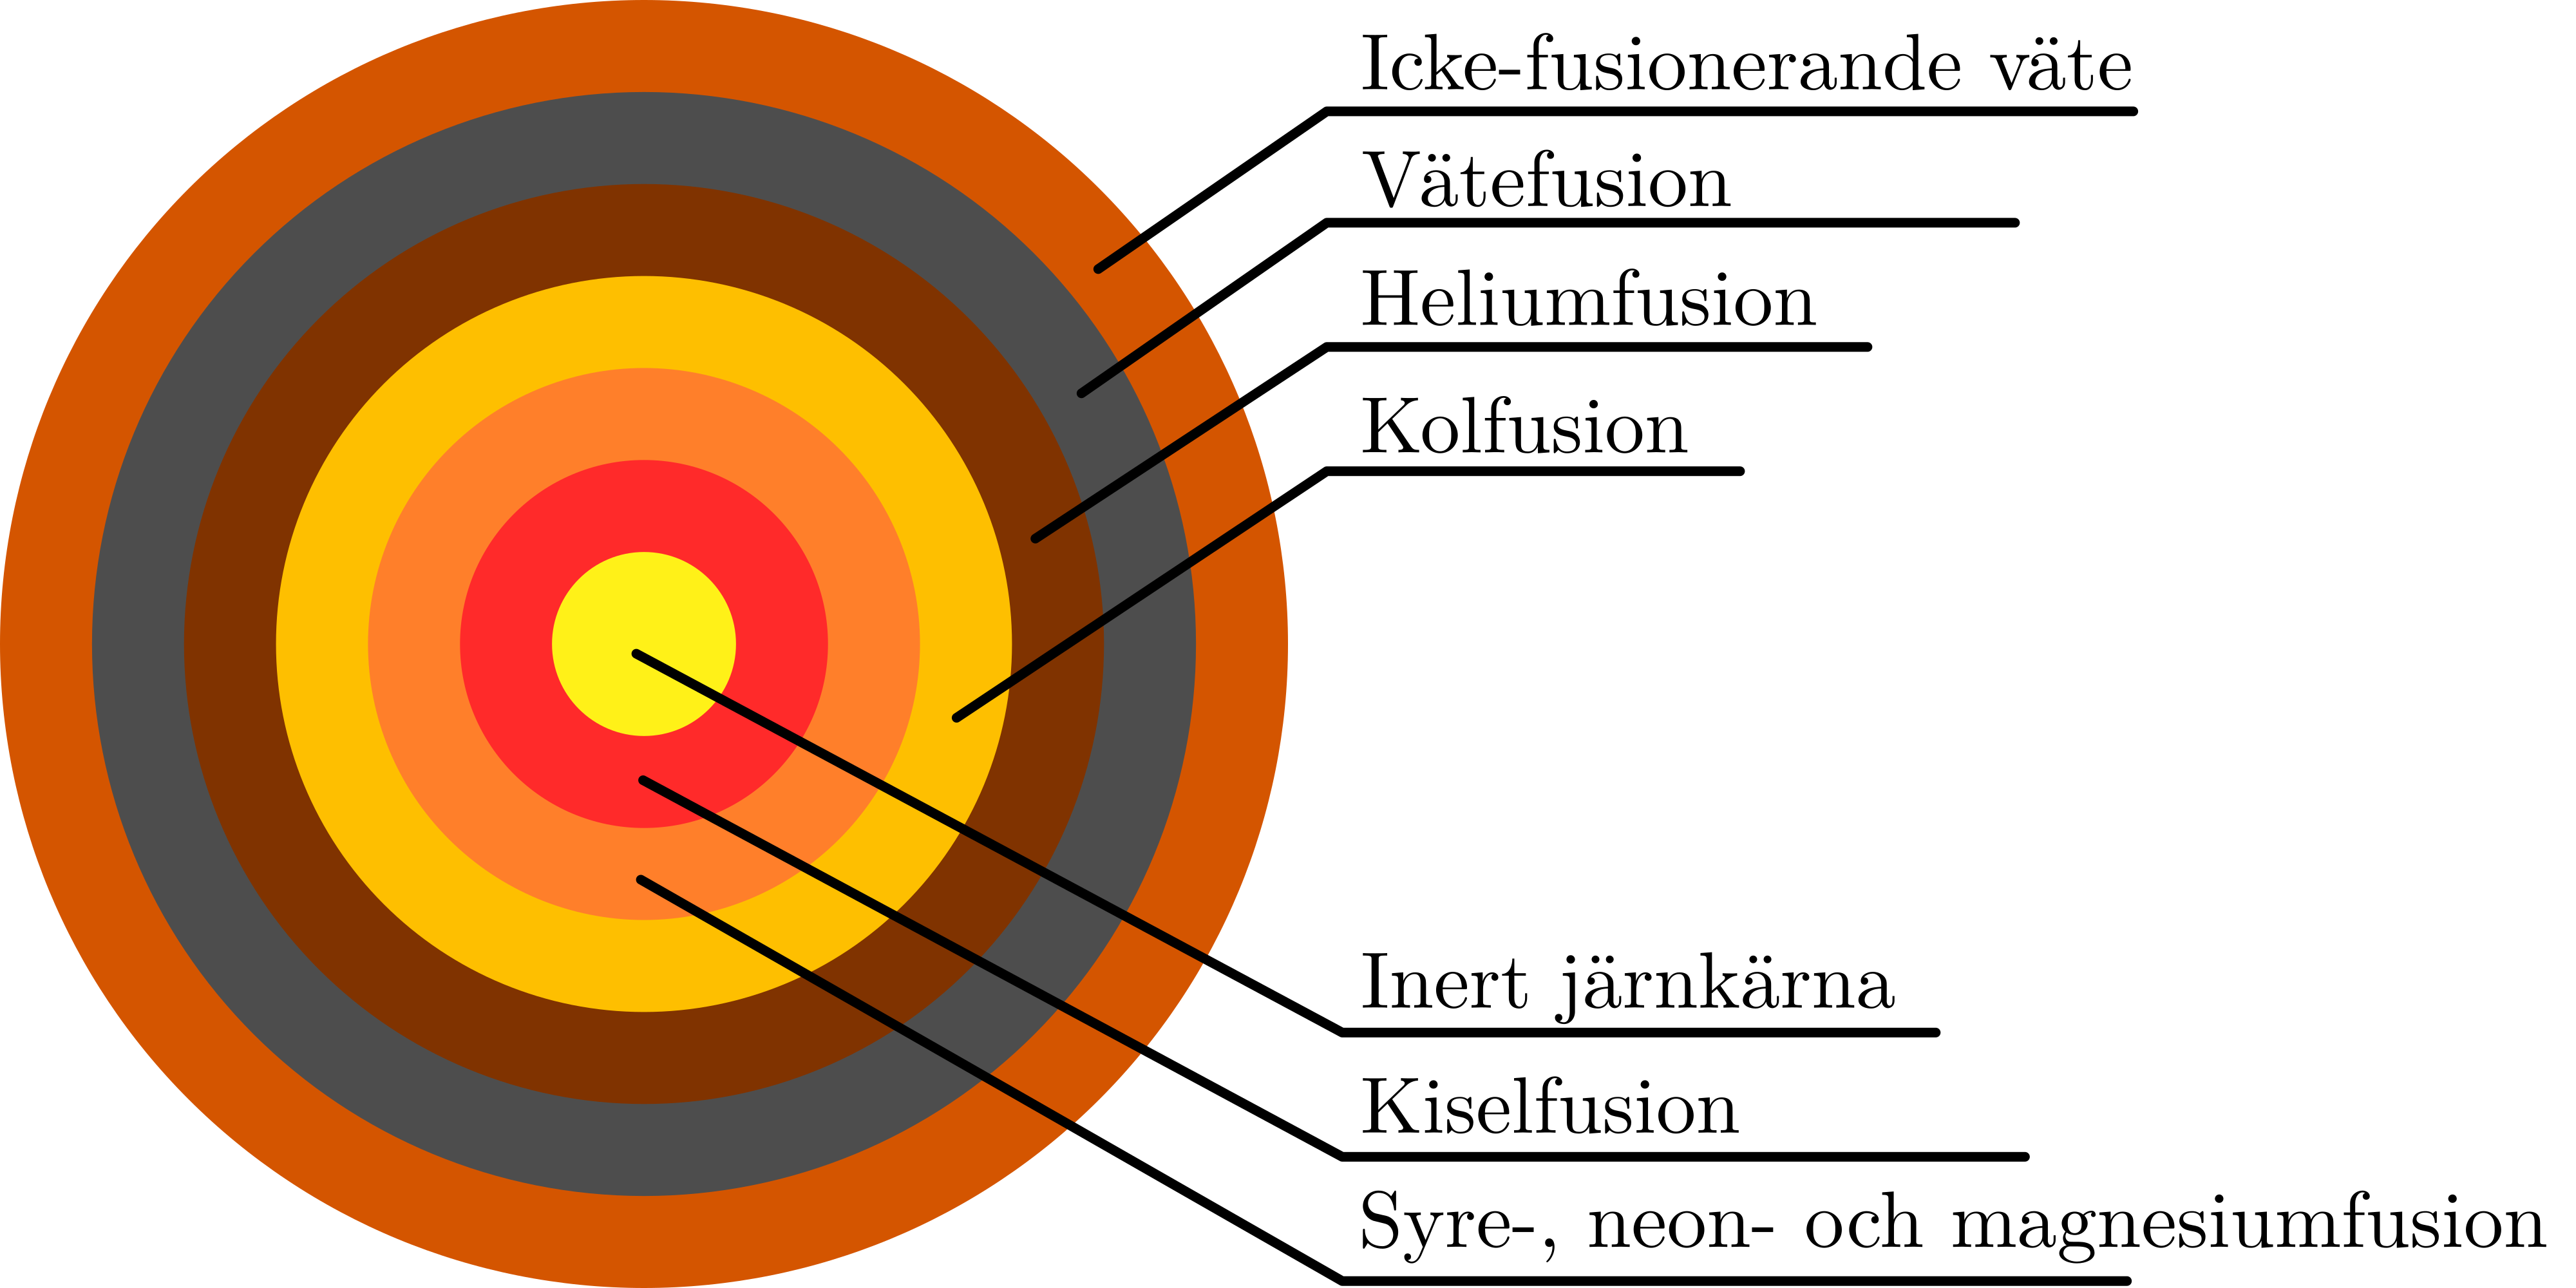
\includegraphics[width=0.8\textwidth]{img/star.png}
    \caption{En massiv, gammal stjärnas inre struktur.}
    \label{fig:star-anatomy}
\end{figure}

\section{Stjärnors livscykel}
En stjärnas liv består i huvudsak av tre steg: (i) födelse, (ii) huvudserie (vätefusion) och (iii) väg till döden. Alla stjärnor föds och lever olika långt på huvudserieen, dock dör olika stjärnor på olika sätt.

Stjärnor föds genom att gas från rymden samlas tack vare gravitation på en punkt. När denna gasklump blir massiv nog, det vill säga cirka \qty{0.08}{\Mo}, kommer vätefusion att inledas. Då börjar stjärnan dess existens på den så kallade \emph{huvudserieen}. Under denna tid samlas helium som lagras i kärnan. Vad som händer sen beror på hur massiv stjärnan är, det vill säga vilka element den kommer kunna fusionera.

\subsection{Små stjärnor}
Små stjärnor mindre än ca \qty{0.5}{\Mo} kommer aldrig att kunna fusionerna helium då de saknar massan för att skapa tillräckligt med tryck. De kommer stanna på huvudserieen länge, upp till flera biljarder ($10^{12}$) år. Det innebär också att inga sådana stjärnor har dött än, för att denna tid är längre än universums livstid. När de har bränt upp allt väte kommer de att kollapsa till en vit dvärg (se \vref{sec:white-dwarfs}).

\subsection{Medelstora stjärnor}
Stjärnor mellan \qtyrange{0.5}{2.25}{\Mo} har nog med massa för att fusionera helium. De kommer först att ansamla helium i kärnan utan att fusionera det då det inte är varmt nog. Till slut kommer heliumet bli så mycket att det tvingar ut vätet och stjärnan får en icke-fusionerande kärna med ett lager av vätefusion runt som tillför nytt helium hela tiden. Detta orsakar att stjärnan växer till att bli mycket större och blåsa iväg en stor andel av sin yttre massa. Därefter kallas stjärnan för en \emph{röd jätte}. Solen kommer till slut att bli en röd jätten, och då kommer den bli \num{250} ggr. större och tappa \qty{30}{\percent} av sin massa.

Till slut blir kärnan stor nog för att fusionerna helium och då kommer denna fusion plötsligt att börja eftersom temperaturen nått gränsen för heliumfusion och allt helium börjar direkt att fusionera. Detta heter \emph{helium flash}. Då krymper också stjärnan och blir mycket varmare på ytan.

När nog med kol bildats från helium kommer även heliumet flytta ut till ett skikt runt den varma, men icke-fusionerande kolkärnan precis som vätet gjorde innan. Kolet går dock inte att fusionera längre vid denna massa (energi/värme), så stjärnan kommer över tid att förbruka sitt bränsle.

\subsection{Stora stjärnor}
För stjärnor \qtyrange{2.25}{4}{\Mo} händer samma sak som ovan, men heliumfusion börjar lite smått redan innan skikten bildas och stjärnan går över till att vara en jätte. Detta beror på att stjärnan når gränsen till heliumfusion innan heliumet lyckas bilda en icke-fusionerande kärna men saknar densiteten att fusionera fullskaligt.

\subsection{De största stjärnorna}
Stjärnor \qty{>9}{\Mo} blir först blåa jättar och sedan röda jättar. Om massan är \qty{>40}{\Mo} kommer stjärnan aldrig blir röd jätte eftersom den tappar för mycket massa. Om större stjärnor uppfyller massan för att fusionera element tyngre än helium kommer de utvecklas längre än de mindre stjärnorna. Exempelvis kommer kolkärnan att fusioneras efter ett tag, med helium och väteskikt runt. Sedan kommer det att bli tyngre och tyngre element i mitten när temperaturen successivt ökar. Vid järn upphör energipositiv fusion och stjärnan kollapsar under sin egna vikt.

\subsection{Kollaps}
När fusion upphör kommer stjärnan att kollapsa. Detta är för att det enda som höll upp stjärnan under dess egna vikta var trycket från den pågående fusionen. För små stjärnor blir det som sagt direkt en vit dvärg (\vref{sec:white-dwarfs}). Detta gäller för massor \qty{<1.4}{\Mo}. För stjärnor med \qtyrange{1.4}{4}{\Mo} kommer det bli en supernova, en stor explosion, sedan en neutronstjärna kvar. För större stjärnor blir det i stället ett svart hål då neutronstjärnan inte klarar att hålla upp sig själv under dess egna vikt.


\section{Stjärnors ljus}
Stjärnor lyser eftersom de är varma. Alla föremål som har en temperatur större än absoluta nollpunkten avger ljus av något slag ($\qty{0}{K} = \qty{-273.15}{\degreeCelsius}$). Till och med du som läser detta lyser! (dock osynligt.) Denna strålning heter svartkroppsstrålning och avger lite av alla våglängder av ljus. Den heter ''svartkropp'' eftersom det är strålningen en perfekt, svart kropp skulle avge vid en given temperatur. En perfekt, svart kropp här innebär ett ogenomskinligt föremål som inte reflekterar något ljus.

Ljuset som avges kommer att följa en särskild fördelning som heter \emph{Plancks lag}. Fördelningen beror endast på föremålets temperatur. Ett exempel på hur fördelning av svartkroppsstrålning ser ut för olika temperaturer finns i \cref{fig:planck-distribution}. Verkligheten är såklart inte lika perfekt som grafen, men följer den väldigt nära. Svartkroppsstrålning uttrycks ofta som ''spectral radiance'' och ges av denna komplicerade formel:
\begin{equation}
    B(\nu, T) = \frac{2h\nu^3}{c^2} \frac{1}{e^{\frac{h\nu}{kT}} - 1}
    \label{eq:planck-distribution}
\end{equation}
där $h$ är Plancks konstant och $k$ är Boltzmanns konstant. Formeln beror på frekvensen $\nu$ och temperaturen $T$ i Kelvin.

\begin{figure}[h!]
    \centering
    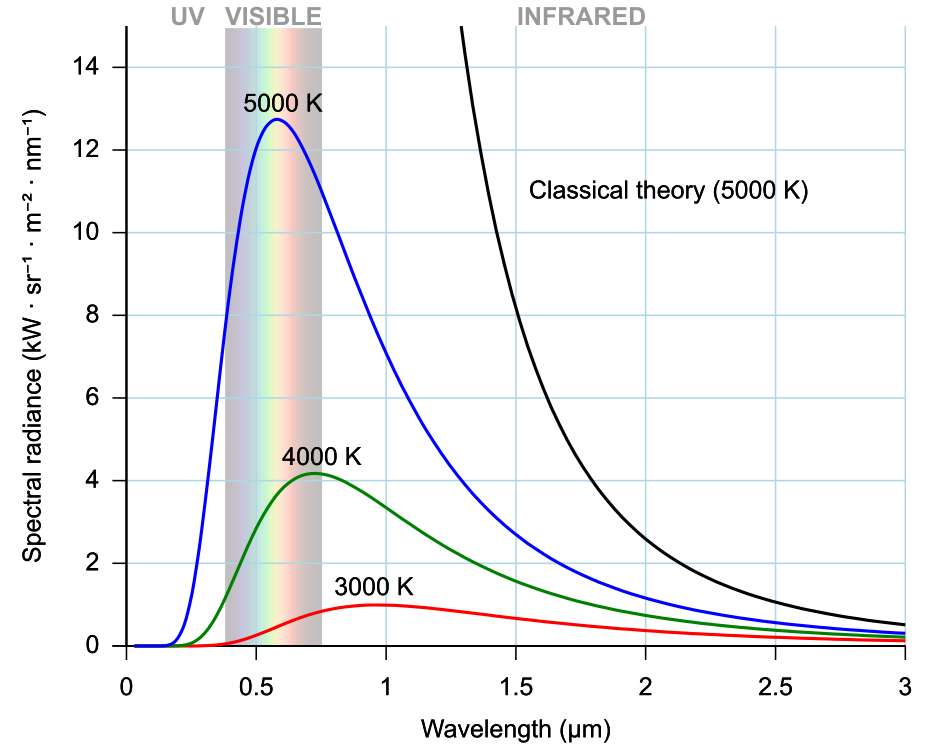
\includegraphics[width=0.75\textwidth]{img/Black_body.png}
    \caption{Plancks lag för olika temperaturer. Y-axeln visar ''ljusstyrka för den specifika våglängden sett på en enhet av föremålets yta'' och x-axeln visar våglängd. Mer specifikt visar y-axeln effekt per enhet area, per enhet rymdvinkel, per enhet våglängd [\unit[per-mode=power]{\watt\per\steradian\per\meter\squared\per\hertz}].}
    \label{fig:planck-distribution}
\end{figure}

Som ni säkert märkt i grafen, finns det en tydlig topp för varje temperatur. Denna topp flyttar sig till ljus med högre och högre energi när temperaturen ökar. Det vill säga att den blir ''blåare''. Man kan beräkna denna topp mycket enklare än hela grafen med Wiens förskjutningslag:
\begin{equation}
    \lambda_\text{max} = \frac{b}{T}
    \label{eq:wien-displacement}
\end{equation}
där $b$ är Wiens förskjutningskonstant och $T$ är temperaturen i Kelvin.

Det är denna våglängd som primärt avgör färgen på ett varmt föremål. Kolla exempelvis hur vi anger lampors färger med temperatur, det beror på att glödlampor generar sitt ljus genom svarkroppsstrålning från glödtråden. Likaså kan vi definiera stjärnors färg som deras våglängdstopp baserat på deras temperatur.

\section{Olika typer av stjärnor}
Man brukar dela in stjärnor på två egenskaper: temperatur och luminositet. Luminositet är kort och gott effekten av ljusstrålningen som stjärnorna skickar ut. Varje foton har nämligen en egen energi som är proportionell mot dess frekvens och ges som
\begin{equation}
    E = hf
    \label{eq:photon-energy}
\end{equation}
där $h$ är Plancks konstant och $f$ är frekvensen i Hertz. Summan av energin i alla fotoner som avges per sekund är stjärnans effekt, alltså luminositet.

Stjärnans temperatur är mer specifikt yttemperaturen. Det vill säga den temperatur som avgör stjärnans färg. En större stjärna kan avge en stor effekt, men fortfarande ha en relativt låg temperatur medan en liten stjärna kan ha en hög temperatur men inte lika hög effekt. Dock tenderar varma stjärnor att vara stora och ljusstarka. Undantaget till detta är vita dvärgar som är väldigt små, har låg luminositet men är ändå väldigt varma.

Man brukar representera dessa kärnegenskaper i ett diagram som heter ett \emph{Hertzsprung-Russell-diagram} (HR-diagram). Där finns också ekvivalenta storheter, såsom magnitud och spektralklass (se nedan) med. Ett exempel på ett sådant diagram finns i \cref{fig:hr-diagram}. Det vikta att ta med från det diagrammet är att man kan få samma temperatur --- samma färg --- vid olika luminositeter (effekter). Detta beror bland annat på storlek, då en röd jätte kan ha samma temperatur som en liten huvudseriestjärna men ändå vara mycket mer ljusstark. Notera även att stjärnorna i huvudserieen förklarat innan hår till ett särskilt band på diagrammet. Det är detta band som kallas huvudserieen och stjärnorna fick sitt namn av bandet. Lika så finns jättarna och de vita dvärgarna inritade.

\begin{figure}[h!]
    \centering
    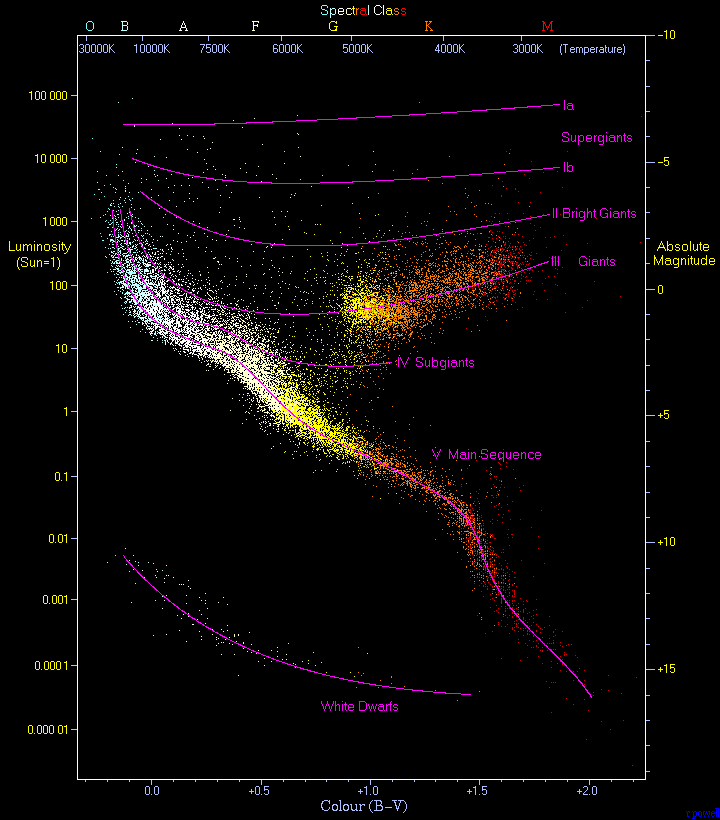
\includegraphics[width=0.75\textwidth]{img/HRDiagram.png}
    \caption{Ett HR-diagram.}
    \label{fig:hr-diagram}
\end{figure}

\subsection{Magnitud}
Det finns en logaritmisk skala som heter \emph{Magnitud} som används för att klassificera olika ljusstyrkor. Skillnaden från luminositet är att magnitud beror på avstånd och hur mycket ljus som har absorberats eller spridits på vägen. Skalan är inverst logaritmisk och är definierad så att en stjärna med magnitud 1 är 100 gånger ljusare än en stjärna med magnitud 6. Alltså är varje steg på skala $\sqrt[5]{100} \approx \num{2.512}$ gånger ljusare än föregående steg. Att den är invers betyder att högre magnitud betyder svagare ljusstyrka. De ljusstarkaste stjärnorna har negativ magnitud.

Man delar också upp magnitudskalan i \emph{skenbar-} och \emph{absolut} magnitud. Skenbar magnitud är hur ljusstark föremålet ser ut från där vi befinner oss. Solen har exempelvis en skenbar magnitud på $-27$. Absolut magnitud, åtminstone för stjärnor, är definierat som deras ljusstyrka på ett av stånd av \qty{10}{pc} (parsec, $\qty{1}{pc}\approx \qty{3.26}{ly}$) från stjärnan med absorption och spridning av ljuset längs vägen försummad. Absolut magnitud är alltså bara ett omständigt, omskalat sätt att jämföra stjärnors luminositet och yta vilket är de två faktorerna som påverkar ljusstyrka.

\subsection{Spektralklass}
Vi har också delat in stjärnors temperaturer i så kallade \emph{spektralklasser}. Varje klass har en karakteristisk färg, alltså temperatur. Klasserna är O, B, A, F, G, K, och M från varmast till kallast. Deras färger och temperaturer finns i \cref{tab:spectral-classes}. Klasserna är i praktiken även underdelade dessa bokstäver, men overgripande är det dessa bokstäver som gäller. Exempelvis är solen en G-stjärna (specifikt G2V vilket betyder att den ligger på de varma änden av G).

\begin{table}[h!]
    \centering
    \caption{Spektralklasser och deras upplevda färger (kromaticitet). Observera att detta inte är samma sak som $\lambda_\text{max}$ i Wiens förskjutningslag. Även massan de skulle ha om de vara på huvudserieen finns med.}
    \label{tab:spectral-classes}
    \begin{tabular}{c | c | c | c}
        \textbf{Klass} & \textbf{Färg} & \textbf{Temperatur} & \textbf{Huvudseriemassa}\\ \midrule
        O & \cellcolor{Ostar} Blå & \qty{\geq 33000}{K} & \qty{\geq 16}{\Mo} \\
        B & \cellcolor{Bstar} Mörk blå-vit & \qtyrange{10000}{33000}{K} & \qtyrange{2.1}{16}{\Mo} \\
        A & \cellcolor{Astar} blå-vit & \qtyrange{7300}{10000}{K} & \qtyrange{1.4}{2.1}{\Mo} \\
        F & \cellcolor{Fstar} typ vit & \qtyrange{6000}{7300}{K} & \qtyrange{1.04}{1.4}{\Mo} \\
        G & \cellcolor{Gstar} gul-vit & \qtyrange{5300}{6000}{K} & \qtyrange{0.8}{1.04}{\Mo} \\
        K & \cellcolor{Kstar} gul-orange & \qtyrange{3900}{6300}{K} & \qtyrange{0.45}{0.8}{\Mo} \\
        M & \cellcolor{Mstar} orange & \qtyrange{2300}{3900}{K} & \qtyrange{0.08}{0.45}{\Mo} \\
    \end{tabular}
\end{table}

\subsection{Vita dvärgar}
\label{sec:white-dwarfs}
Vita dvärgar är kvarlevorna efter stjärnor vars massa vid döden är \qty{\leq 1.4}{\Mo}\footnote{Chandrasekhargränsen. Det är den största möjliga massan för en icke-fusionerande stjärna innan den kollapsar vidare till en neutronstjärna.} kollapsar. De är en typ av icke-fusionerande stjärna. De består av den lilla massa som blir kvar av en stjärna efter dess jätte-fas eller efter dess supernova. Då det inte finns någon fusion kvar i stjärnan hålls de från kollaps av endast trycket från materialet de består av. Detta innebär också att det kyls ner över tid då fusion inte tillför ny värme. Till slut kommer den att endast vara en klump av metaller och is som heter en svart dvärg. Detta tar dock mycket längre tid än universums nuvarande livstid, så det är mycket tid kvar tills de första svarta dvärgarna kommer bildas.

\subsection{Neutronstjärnor}
Om en stjärna som har en massa mellan \qtyrange{1.4}{2.1}{\Mo} dör kommer den att kollapsa till en neutronstjärna. Dessa heter så eftersom de består nästan helt av neutroner. I detta massintervall är gravitationen så stark utan fusionstrycket att elektroner trycks in i protoner som sedan blir till neutroner via en process som heter invers-$\beta$-sönderfall. Till skillnad för vanlig $\beta$-sönderfall där en neutron blir till en elektron och en proton i radioaktiva ämnen. Det enda som håller stjärnans form är den så kallade \emph{neutrondegererationstrycket} som alstras eftersom två identiska neutroner inte gärna vill existera på samma plats samtidigt.

Neutronstjärnor har heller ingen fusion och kommer fortsätta existera så länge de har kvarvarande värme. Likt vita dvärgar, kommer de till slut att kylas ner och sluta stråla men de kan existera i princip för evigt så länge inget påverkar dem. Det allra vanligaste döden för neutronstjärnor är dock att de kollapsar till svarta hål genom att samla massa från närliggande föremål som ramlar in i deras gravitation eller genom att krocka med en annan stjärna. De kan också ''suga'' massa från deras partnerstjärna i binära system.

\section{Svarta hål}
Neutronstjärnor med en massa större än ca \qty{2.1}{\Mo}\footnote{Tolman-Oppenheimer-Volkoff gränsen. En otydlig gräns för den största möjliga neutronstjärnan.} är för stora för att klara av att existera under sin egna vikt. Degenerationstrycket är inte starkt nog för att motstå tyngdkraften, så stjärnan kollapsar med all sin massa i en enstaka, oändligt liten punkt: en \emph{singularitet}. En punkt med i princip oändlig densitet, dock finit massa, har så stark gravitation att inte ens ljus kan rymma. Det är därifrån namnet ''svart hål'' kommer ifrån.

Då ljus inte kan rymma från svarta hål, kan vi heller inte se dem eftersom ljus inte kan reflekteras eller strålas ut från dem. Vi kan dock se effekterna av dem, till exempel när de suger in massa från en partnerstjärna i ett binärt system. Vi kan också observera hur ljus böjs runt dem tack vare deras starka gravitation. Svarta hål brukar ofta ha en ring med materia runt som heter en \emph{ackretionsskiva}. Den skivan sugs långsamt in i hålet och blir under processen väldigt varm och därmed lyser.

Svarta hål har en så kallad \emph{händelsehorisont}. Efter denna gräns är det inte längre möjligt för varken ljus eller föremål med massa att komma iväg. De kommer i stället att sugas in i och bli en del av singulariteten. Händelsehorisonten börjar vid den så kallade \emph{Schwarzschildradien} för ett icke-roterande svart hål. Det är avståndet från en punkt med en massa där ljus inte kan rymma, ifall massan är en singularitet. Den ges som
\begin{equation}
    r_s = \frac{2Gm}{c^2},
    \label{eq:schwarzschild-radius}
\end{equation}
där $G$ är gravitationskonstanten, $m$ är massan och $c$ är ljusets hastighet.

Likt allt stellärt material kommer även svarta hål att dö till slut. Dock dör de på mycket annorlunda sätt från neutronstjärnor och vita dvärgar. De strålar hela tiden ut så kallad \emph{Hawkingstrålning}. Det kostar svarta hål energi, och därav massa. Ju större massa desto mer strålning. Till slut, efter mycket lång tid kommer all massa att förbrukas till Hawkingstrålning och det svarta hålet att försvinna.